\section{The Sphere Function}
\label{sec:app:test:sphere}
  The sphere function serves as a prominent benchmark problem in the realm of 
  optimization algorithms.
  This convex function's simplicity and well-defined nature make it ideal for
  gauging the performance of such algorithms.
  
  \begin{definition}[Sphere Function]
    \label{def:app:test:sphere}
    The \emph{sphere function}, denoted as \(f: \mathbb{R}^n \rightarrow 
    \mathbb{R}\), is formally described as:
  
    \begin{equation}
      \label{eq:app:test:sphere}
      f(\mathbf{x}) = \sum_{i=1}^{n} \mathbf{x}_i^2
    \end{equation}
      
    Herein:
  
    \begin{itemize}
      \item \(n \in \mathbb{N}\) signifies the number of dimensions.
      \item \(\mathbf{x}_i \in \mathbb{R}\) represents the \(i\)-th element of 
        the vector \(\mathbf{x}\).
    \end{itemize}
  \end{definition}

  The global minimum of the sphere function occurs at \(f(\mathbf{x}^*) = 0\) 
  with the input vector \(\mathbf{x}^* = (0,\, \ldots,\, 0)\).
  The contour and surface plots showcasing the behavior of the sphere function
  for a two-dimensional input (\(n = 2\)) are illustrated in 
  \vref{fig:app:test:sphere}.

  \begin{figure}[ht!]
    \centering
    \begin{subfigure}[b]{0.4\textwidth}
      \centering
      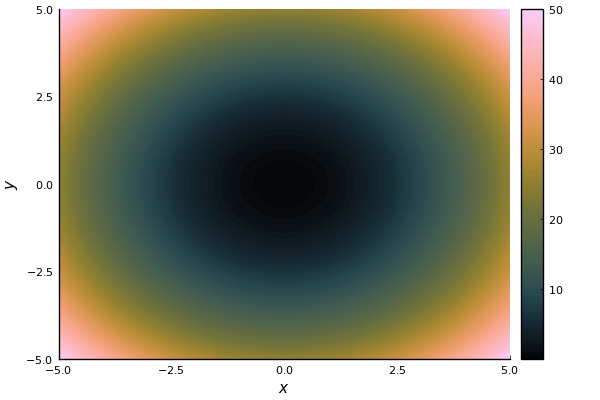
\includegraphics[width=\textwidth]{img/test_functions/sphere_contour.png}
    \end{subfigure}
    \hfill
    \begin{subfigure}[b]{0.4\textwidth}
      \centering
      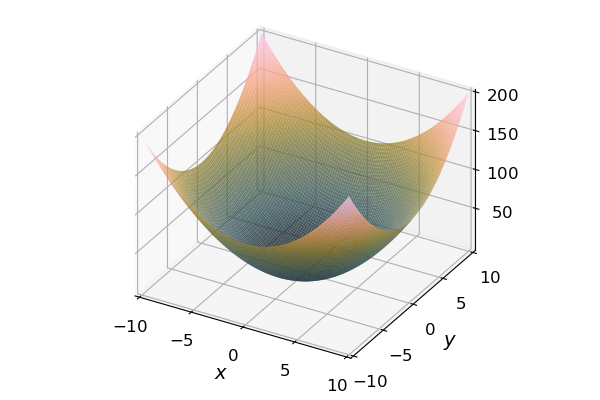
\includegraphics[width=\textwidth]{img/test_functions/sphere_surface.png}
    \end{subfigure}
    \caption{Visual Representation of the Sphere Function with \(n = 2\)}
    \label{fig:app:test:sphere}
  \end{figure}
